\documentclass[12pt]{article}
\twocolumn
\usepackage{graphicx}
\usepackage[none]{hyphenat}
\usepackage{graphicx}
\usepackage{listings}
\usepackage[english]{babel}
\usepackage{graphicx}
\usepackage{caption} 
\usepackage{booktabs}
\usepackage{array}
\usepackage{amssymb} % for \because
\usepackage{amsmath}   % for having text in math mode
\usepackage{extarrows} % for Row operations arrows
\usepackage{listings}
\usepackage[utf8]{inputenc}
\lstset{
  frame=single,
  breaklines=true
}
\usepackage{hyperref}
  
%Following 2 lines were added to remove the blank page at the beginning
\usepackage{atbegshi}% http://ctan.org/pkg/atbegshi
\AtBeginDocument{\AtBeginShipoutNext{\AtBeginShipoutDiscard}}


%New macro definitions
\newcommand{\mydet}[1]{\ensuremath{\begin{vmatrix}#1\end{vmatrix}}}
\providecommand{\brak}[1]{\ensuremath{\left(#1\right)}}
\newcommand{\solution}{\noindent \textbf{Solution: }}
\newcommand{\myvec}[1]{\ensuremath{\begin{pmatrix}#1\end{pmatrix}}}
\providecommand{\norm}[1]{\left\lVert#1\right\rVert}
\providecommand{\abs}[1]{\left\vert#1\right\vert}
\let\vec\mathbf

\begin{document}

\begin{center}
\title{\textbf{LINE}}
\date{\vspace{-5ex}} %Not to print date automatically
\maketitle
\end{center}

\section{11$^{th}$ Maths - EXERCISE-10.2}
\begin{enumerate}
\item Passing through the point (– 4, 3) with slope $\frac{1}{2}$
\end{enumerate}
\section{SOLUTION}
Given points are (-4,3), and slope $m=\frac{1}{2}$

The line formula in matrix form
\begin{align}
n^\top x&=c\\
\end{align}
\begin{align}
n&=\myvec{m\\-1}\\
&=\myvec{\frac{1}{2}\\-1}\\
c&=\frac{mx_1-y_1}{2}\\
&=2 \myvec{\frac{1}{2}\times-4-3}\\
&=\frac{-10}{2}\\
&=-5
\end{align}

\begin{align}
n^\top x&=c\\
\myvec{\frac{1}{2}\\-1}^\top x&=-5\\
&=x-2y=-10\\
\implies x-2y+10=0
\end{align} 
\section{Figure}
\begin{figure}[h]
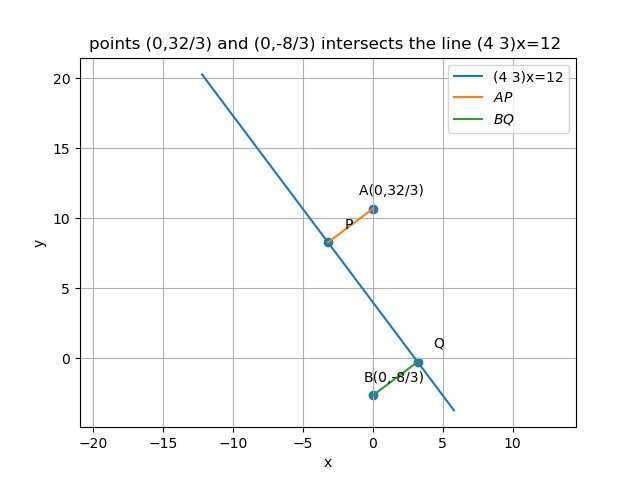
\includegraphics[width=\columnwidth]{fig.png}
\caption{line}
		\label{fig:Figure}
\end{figure}
\end{document}